\usepackage{graphicx}
\usepackage{tikz}
\usetikzlibrary{arrows.meta,positioning,fit,calc,shapes.geometric}
\tikzset{
  umlbox/.style={draw, rounded corners=2pt, align=center, minimum height=7mm, inner sep=3pt, font=\small},
  umlsmallbox/.style={draw, rounded corners=2pt, align=center, minimum height=6mm, inner sep=2pt, font=\scriptsize},
  packagebox/.style={draw, rounded corners=2pt, align=center, inner sep=5pt, font=\small},
  umllifeline/.style={draw, align=center, minimum width=20mm, minimum height=7mm, inner sep=2pt, font=\scriptsize},
  umlmsg/.style={-{Latex[length=2mm]}, line width=0.45pt},
  umlreturn/.style={-{Latex[length=2mm]}, dashed, line width=0.45pt},
  umlrealize/.style={-{Triangle[open,length=3mm,width=3mm]}, dashed, line width=0.45pt},
  umlinherit/.style={-{Triangle[open,length=3mm,width=3mm]}, line width=0.45pt}
}
\newcommand{\ExamPhysicalPackageDiagram}[1]{%
\begin{center}
\resizebox{0.95\linewidth}{!}{%
\begin{tikzpicture}[node distance=22mm]
\node[packagebox] (client) {
\begin{tabular}{c}
\textbf{客户端 / 浏览器}\\
html\\
css\\
javascript\\
presentation
\end{tabular}};
\node[packagebox, right=26mm of client] (server) {
\begin{tabular}{c}
\textbf{服务器端}\\
controller/api\\
service 逻辑层\\
repository 数据层接口\\
domain/entity\\
modules\\
#1\\
database
\end{tabular}};
\draw[umlmsg] (client.east) -- node[above,align=center,font=\small] {HTTP + REST API + JSON} (server.west);
\end{tikzpicture}}
\end{center}}
\newcommand{\ExamDetailedSequenceDiagram}[5]{%
\begin{center}
\resizebox{\linewidth}{!}{%
\begin{tikzpicture}
\node[umllifeline] (user) at (0,0) {User};
\node[umllifeline] (controller) at (3,0) {Controller};
\node[umllifeline] (service) at (6,0) {#2};
\node[umllifeline] (mainRepo) at (9,0) {#4};
\node[umllifeline] (domain) at (12,0) {Strategy / Domain};
\node[umllifeline] (external) at (15,0) {ExternalService};
\node[umllifeline] (relatedRepo) at (18,0) {#5};
\foreach \p in {user,controller,service,mainRepo,domain,external,relatedRepo} {
  \draw[dashed] (\p.south) -- ++(0,-7.9);
}
\draw[umlmsg] (0,-0.7) -- node[above,font=\scriptsize] {submit #1 request} (3,-0.7);
\draw[umlmsg] (3,-1.4) -- node[above,font=\scriptsize] {#3(command)} (6,-1.4);
\draw[umlmsg] (6,-2.1) -- node[above,font=\scriptsize] {query domain object} (9,-2.1);
\draw[umlreturn] (9,-2.8) -- node[above,font=\scriptsize] {domain object} (6,-2.8);
\draw[umlmsg] (6,-3.5) -- node[above,font=\scriptsize] {check rules and calculate result} (12,-3.5);
\draw[umlmsg] (6,-4.2) -- node[above,font=\scriptsize] {call external interface if needed} (15,-4.2);
\draw[umlreturn] (15,-4.9) -- node[above,font=\scriptsize] {external result} (6,-4.9);
\draw[umlmsg] (6,-5.6) -- node[above,font=\scriptsize] {save updated entity} (9,-5.6);
\draw[umlmsg] (6,-6.3) -- node[above,font=\scriptsize] {query or update related data} (18,-6.3);
\draw[umlreturn] (6,-7.0) -- node[above,font=\scriptsize] {result DTO} (3,-7.0);
\draw[umlreturn] (3,-7.7) -- node[above,font=\scriptsize] {HTTP response} (0,-7.7);
\end{tikzpicture}}
\end{center}}
\newcommand{\ExamStrategyDiagram}[5]{%
\begin{center}
\resizebox{\linewidth}{!}{%
\begin{tikzpicture}
\node[umlbox] (context) at (0,1.8) {#1};
\node[umlbox] (strategy) at (6.5,1.8) {\textless\textless interface\textgreater\textgreater\\#2};
\node[umlsmallbox] (a) at (0,-1.0) {#3};
\node[umlsmallbox] (b) at (6.5,-1.0) {#4};
\node[umlsmallbox] (c) at (13.0,-1.0) {#5};
\draw[umlmsg,dashed] (context.east) -- node[above,font=\scriptsize] {depends on} (strategy.west);
\draw[umlrealize] (a) -- (strategy);
\draw[umlrealize] (b) -- (strategy);
\draw[umlrealize] (c) -- (strategy);
\end{tikzpicture}}
\end{center}}
\newcommand{\ExamObserverDiagram}{%
\begin{center}
\resizebox{0.9\linewidth}{!}{%
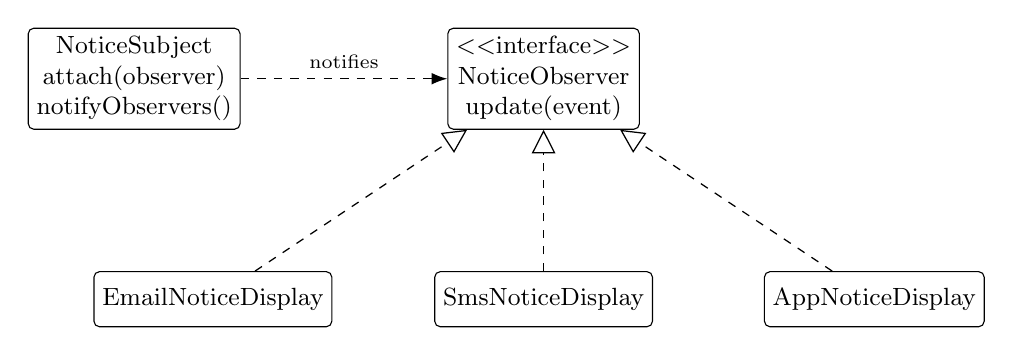
\begin{tikzpicture}
\node[umlbox] (subject) at (0,1.8) {NoticeSubject\\attach(observer)\\notifyObservers()};
\node[umlbox] (observer) at (5.2,1.8) {\textless\textless interface\textgreater\textgreater\\NoticeObserver\\update(event)};
\node[umlbox] (email) at (1.0,-1.0) {EmailNoticeDisplay};
\node[umlbox] (sms) at (5.2,-1.0) {SmsNoticeDisplay};
\node[umlbox] (app) at (9.4,-1.0) {AppNoticeDisplay};
\draw[umlmsg,dashed] (subject.east) -- node[above,font=\scriptsize] {notifies} (observer.west);
\draw[umlrealize] (email) -- (observer);
\draw[umlrealize] (sms) -- (observer);
\draw[umlrealize] (app) -- (observer);
\end{tikzpicture}}
\end{center}}
\newcommand{\ExamAbstractFactoryDiagram}{%
\begin{center}
\resizebox{0.95\linewidth}{!}{%
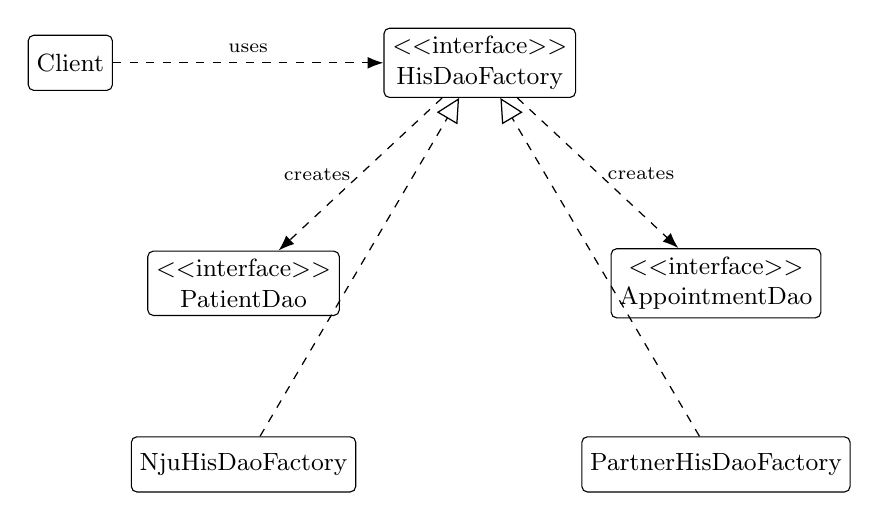
\begin{tikzpicture}
\node[umlbox] (client) at (-2.2,2.0) {Client};
\node[umlbox] (factory) at (3,2.0) {\textless\textless interface\textgreater\textgreater\\HisDaoFactory};
\node[umlbox] (patientDao) at (0,-0.8) {\textless\textless interface\textgreater\textgreater\\PatientDao};
\node[umlbox] (appointmentDao) at (6,-0.8) {\textless\textless interface\textgreater\textgreater\\AppointmentDao};
\node[umlbox] (nju) at (0,-3.1) {NjuHisDaoFactory};
\node[umlbox] (partner) at (6,-3.1) {PartnerHisDaoFactory};
\draw[umlmsg,dashed] (client) -- node[above,font=\scriptsize] {uses} (factory);
\draw[umlmsg,dashed] (factory) -- node[left,font=\scriptsize] {creates} (patientDao);
\draw[umlmsg,dashed] (factory) -- node[right,font=\scriptsize] {creates} (appointmentDao);
\draw[umlrealize] (nju) -- (factory);
\draw[umlrealize] (partner) -- (factory);
\end{tikzpicture}}
\end{center}}
\newcommand{\ExamIteratorDiagram}{%
\begin{center}
\resizebox{0.9\linewidth}{!}{%
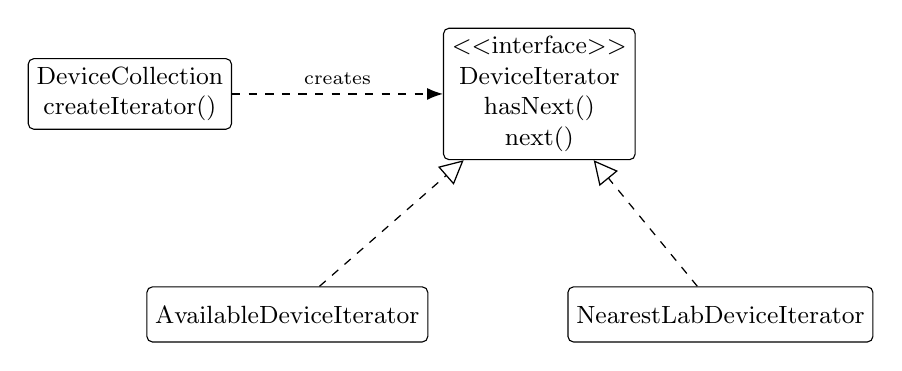
\begin{tikzpicture}
\node[umlbox] (collection) at (0,1.8) {DeviceCollection\\createIterator()};
\node[umlbox] (iterator) at (5.2,1.8) {\textless\textless interface\textgreater\textgreater\\DeviceIterator\\hasNext()\\next()};
\node[umlbox] (available) at (2.0,-1.0) {AvailableDeviceIterator};
\node[umlbox] (nearest) at (7.5,-1.0) {NearestLabDeviceIterator};
\draw[umlmsg,dashed] (collection) -- node[above,font=\scriptsize] {creates} (iterator);
\draw[umlrealize] (available) -- (iterator);
\draw[umlrealize] (nearest) -- (iterator);
\end{tikzpicture}}
\end{center}}
